\documentclass[oneside,a4paper,12pt]{article}
\usepackage[english,brazilian]{babel}
\usepackage{multicol}
\usepackage{textcomp}
\usepackage[alf]{abntex2cite}
\usepackage[utf8]{inputenc}
\usepackage[T1]{fontenc}
\usepackage{amsmath,amssymb,exscale}
\usepackage[top=20mm, bottom=20mm, left=20mm, right=20mm]{geometry}%margens cima, baixo, esquerda direita
\usepackage{framed}
\usepackage{booktabs} %Pacote para deixar tabelas mais bonitas.
\usepackage{color} %Pacote de Cores
\usepackage{hyperref} %Pacotes para Hiperlinks
\usepackage{graphicx} %Pacote de imagens
\graphicspath{{./Figuras/}}%Direciona as imagens para uma pasta chamada "Figuras" (uso isso para organizar. Uma vez que todas as imagens vao ficar em uma pasta isolada)    
\definecolor{shadecolor}{rgb}{0.8,0.8,0.8}

%FAZ EDICOES AQUI (somente no conteudo que esta entre entre as ultimas  chaves de cada linha!!!)
\newcommand{\universidade}{Universidade Estadual de Londrina}
\newcommand{\centro}{Centro de Ciências Exatas}
\newcommand{\departamento}{Departamento Matemática}
\newcommand{\curso}{Física}
\newcommand{\professores}{Matheus Pimenta}
\newcommand{\disciplina}{Cálculo I - 1MAT096}
%\newcommand{\tema}{Lista 01}
%\newcommand{\turma}{MA31G}
%\newcommand{\data}{Março de 2019}%{\today}
%\newcommand{\tempodeaula}{30 minutos}
%\newcommand{\prerequisitos}{Matrizes, Transformações Lineares e Bases}
%ATE AQUI !!!	

\begin{document}
	\pagestyle{empty}
	
	\begin{center}
		
\includegraphics[width=\linewidth/2]{logo.jpg}%LOGOTIPO DA INSTITUICAO
	 	\vspace{2pt} 	
		
		\universidade
		\par
		\centro
		\par
		\departamento
		\par
	%	Curso de \curso
		\par
		\vspace{12pt}
		\LARGE \textbf{Lista 03}
		
	\end{center}
	
	\vspace{12pt}
	
	\begin{tabular}{ |l|p{12cm}| }
		
		\hline
		\multicolumn{2}{|c|}{\textbf{Dados de Identificação}} \\
		\hline
		Professor:         &    \professores           \\
		\hline
		Disciplina:        &    \disciplina          \\
		\hline
	%	Tema:              &    \tema                \\
	%	\hline
	%	Pré-requisito	:  &    \prerequisitos         \\
	%	\hline
		Aluno:             &                   \\
	%	\hline
	%	Data:              &    \data                \\
	%	\hline
	%	Duração da aula:   &    \tempodeaula         \\
		\hline
		
	\end{tabular}
	\vspace{6pt}
	
	
	\begin{snugshade}
	\end{snugshade}

\begin{enumerate}
	\setcounter{enumi}{37}

	\item Dado o gráfico determine e justifique:
	\begin{figure}[!h]
		\centering
		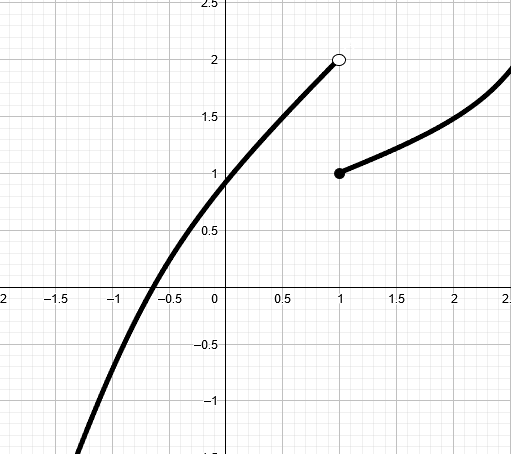
\includegraphics[scale=0.6]{ex1}
		\label{ex1}
	\end{figure}
	\begin{multicols}{2}
	\begin{enumerate}
		\item $\lim\lim\limits_{x\rightarrow 0^{-}}f(x) = 1$
		\item $\lim\lim\limits_{x\rightarrow 0^{+}}f(x) = 1$
		\item $\lim\lim\limits_{x\rightarrow 0}f(x) = 1$
		\item $\lim\lim\limits_{x\rightarrow 1^{-}}f(x) = 2$
		\item $\lim\lim\limits_{x\rightarrow 1^{+}}f(x) = 1$
		\item $\lim\lim\limits_{x\rightarrow 1}f(x) = \nexists$
	\end{enumerate}
	\end{multicols}

	\item Determine os limites conforme indicado:
	\begin{multicols}{2}
	\begin{enumerate}
		\item $\lim\limits_{x\rightarrow \sqrt{5}}3\pi = 3\pi$
		\item $\lim\limits_{x\rightarrow \frac{1}{5}}\frac{2x-3}{5x+1} = -\frac{13}{10}$
		\item $\lim\limits_{x\rightarrow 0}\frac{x^2 - 2x}{x} = 2$
		\item $\lim\limits_{x\rightarrow 2}\frac{x^2 - 4x + 4}{x^2 - 2x} = 0$
		\item $\lim\limits_{x\rightarrow 3}\frac{2x^3 - 6x^2 + x - 3}{x-3} = 19$
	\end{enumerate}
	\end{multicols}

	\item Determine os limites conforme indicado:
	\begin{multicols}{2}
	\begin{enumerate}
		\item $\lim\limits_{x\rightarrow 1}\frac{x^3 - 1}{x-1}=3$
		\item $\lim\limits_{x\rightarrow -1}\frac{-4x+6}{5x-4}=-\frac{10}{9}$
		\item $\lim\limits_{x\rightarrow -1}\sqrt{\frac{2x+5}{2x^2 - 3x}}=\frac{\sqrt{15}}{5}$
		\item $\lim\limits_{x\rightarrow 3}\frac{x-3}{|x-3|}=\nexists$
		\item $\lim\limits_{x\rightarrow 1}\frac{2x+2}{|x+1|}=2$
	\end{enumerate}
	\end{multicols}

	\item Determine os limites conforme indicado:
	\begin{multicols}{2}
	\begin{enumerate}
		\item $\lim\limits_{x\rightarrow 5}\frac{2x - 10}{|x-5|} = \nexists$
		\item $\lim\limits_{x\rightarrow 1^{-}}\frac{2x}{x-1} = -\infty$
		\item $\lim\limits_{x\rightarrow 1^{+}}\frac{2x}{x-1} = + \infty$
		\item $\lim\limits_{x\rightarrow 1}\frac{2x^2 + 5x - 7}{x^2 - x} = 9$
		\item $\lim\limits_{x\rightarrow 5}\frac{-x^2 + 4x + 5}{x^2 - 12x + 35} = 3$
	\end{enumerate}
	\end{multicols}

	\item Determine os limites conforme indicado:
	\begin{multicols}{2}
	\begin{enumerate}
		\item $\lim\limits_{x\rightarrow 9}\frac{\sqrt{x} - 3}{x - 9} = \frac{1}{6}$
		\item $\lim\limits_{x\rightarrow 4}\frac{2x - 8}{\sqrt{x} - 2} = 8$
		\item $\lim\limits_{x\rightarrow 2}\frac{x^2 - 4}{x^3 - 8} = \frac{1}{3}$
		\item $\lim\limits_{x\rightarrow -1}\frac{x^3 + x^2 + 3x + 3}{x+1} = 4$
		\item $\lim\limits_{y\rightarrow -2}\frac{y^3 + 8}{y + 2} = 12$
	\end{enumerate}
	\end{multicols}

	
	\item Determine os limites conforme indicado:
	\begin{multicols}{2}
		\begin{enumerate}
			\item $\lim\limits_{x\rightarrow 6}(5x + 4) = 34$
			\item $\lim\limits_{x\rightarrow -3}(2x^2 - 8x + 4) = 46$
			\item $\lim\limits_{x\rightarrow 0}(-x^2 + 4) = 4$
			\item $\lim\limits_{y\rightarrow -2}(3y^3 + 2y^2 - 5y - 2) = -8$
			\item $\lim\limits_{x\rightarrow -4}(-3x + 7) = 19$
			\item $\lim\limits_{x\rightarrow 2}\frac{5x - 2}{4x + 1} = \frac{8}{9}$
		\end{enumerate}
	\end{multicols}
	
	\item Esboce o gráfico da função $f$ definida por:
	$$f(x) = \begin{cases}
	3 - x \text{ ,se } x < 1 \\
	4	\text{ ,se } x =1 \\
	x^2 + 1 \text{ ,se } x>1 
	\end{cases}
	$$
	\begin{multicols}{3}
	\begin{enumerate}
		\item $\lim\limits_{x\rightarrow 1^{-}}f(x) = 2$
		\item $\lim\limits_{x\rightarrow 1^{+}}f(x) = 2$
		\item $\lim\limits_{x\rightarrow 1}f(x) = 2$
	\end{enumerate}
	\end{multicols}

	\item Determine os limites conforme indicado:
	\begin{multicols}{2}
		\begin{enumerate}
			\item $\lim\limits_{x\rightarrow + \infty}\frac{1}{x^2} = 0$
			\item $\lim\limits_{x\rightarrow + \infty}\frac{4x - 5}{3x - 2} = \frac{4}{3}$
			\item $\lim\limits_{x\rightarrow - \infty}\frac{2x^2 - x + 5}{4x^3 - 1} = 0$
			\item $\lim\limits_{x\rightarrow + \infty}\frac{3x + 4}{\sqrt{2x^2 - 5}} = \frac{3}{2}\sqrt{2}$
			\item $\lim\limits_{x\rightarrow - \infty}\frac{3x+4}{\sqrt{2x^2 - 5}} = -\frac{3}{2}\sqrt{2}$
			\item $\lim\limits_{x\rightarrow + \infty}\frac{2x - x^2}{3x + 5} = \infty$
		\end{enumerate}
	\end{multicols}

	\item Determine os limites conforme indicado:
	\begin{multicols}{2}
		\begin{enumerate}
			\item $\lim\limits_{x\rightarrow 0}\frac{\sin(7x)}{x} = 7$
			\item $\lim\limits_{x\rightarrow 0}\frac{\sin(4x)}{\sin(9x)} = \frac{4}{9}$
			\item $\lim\limits_{x\rightarrow 0}\frac{\sin(\frac{x}{3})}{x} = \frac{1}{3}$
			\item $\lim\limits_{x\rightarrow 0}\frac{\cos(x) - 1}{x^2} = - \frac{1}{2}$
			\item $\lim\limits_{x\rightarrow \frac{\pi}{4}}\frac{\cos(x) - \sin(x)}{\tan(x)-1} = - \frac{\sqrt{2}}{2}$
			\item $\lim\limits_{x\rightarrow  \infty}\left( 1 + \frac{5}{x} \right)^{x} = e^5$
		\end{enumerate}
	\end{multicols}


	\item Determine os limites conforme indicado:
	\begin{multicols}{2}
		\begin{enumerate}
			\item $\lim\limits_{x\rightarrow  \infty}\left( \frac{x - 2}{x} \right)^{x} = e^{-2}$
			\item $\lim\limits_{x\rightarrow  \infty}\left( \frac{x - 2}{x + 4} \right)^{x + 2} = e^{-6}$
			\item $\lim\limits_{x\rightarrow 0}\left( \frac{3^{2x}-1}{x} \right) = 2\ln(3)$
			\item $\lim\limits_{x\rightarrow 0}\frac{2^{3x}-1}{3^{2x}-1} = \frac{3 \ln(2)}{2 \ln(3)}$
			\item $\lim\limits_{x\rightarrow 0}\frac{4^{3x}-1}{4^{2x}-1} = \frac{3}{2}$
			\item $\lim\limits_{x\rightarrow 0}\frac{\sin(x + a) - \sin(a)}{x} = \cos(a)$
		\end{enumerate}
	\end{multicols}

	\item Verifique se as funções definidas a seguir são contínuas nos pontos especificados:
		\begin{enumerate}
			\item $f(x) = \begin{cases}
			x^2 - 3 \text{ ,se } x \leq 2 \\
			5-2x	\text{ ,se } x > 2
			\end{cases}
			$ é contínua em $x=2$. \\ {\bf R:} Sim
			\item $f(x) = \begin{cases}
			x^2 - 6x + 8 \text{ ,se } x \geq 2 \\
			x^2 + x - 6 \text{ ,se } x < 2
			\end{cases}
			$ é contínua em $x = 2$. \\ {\bf R:} Sim
			\item $f(x) = \begin{cases}
			\frac{x^3 - 27}{x-3} \text{ ,se } x \neq 3 \\
			3	\text{ ,se } x = 3
			\end{cases}
			$ é contínua em $x=3$. \\ {\bf R:} Não
			\item $f(x) = \begin{cases}
			\frac{1}{|x-1|}	\text{ ,se } x \neq 1 \\
			1	\text{ ,se } x = 1
			\end{cases}
			$ é contínua em $x=1$. \\ {\bf R:} Não
		\end{enumerate}

	
	\item Suponha que para todo $x$, $|f(x)| \leq x^4$. Calcule $\lim\limits_{x\rightarrow 0}\frac{f(x)}{x}$ \\ {\bf R:} 0
	
	\item Mostre que $\lim\limits_{x\rightarrow 0}x^2.\sin(\frac{1}{x}) = 0$



\end{enumerate}


	
\end{document}
